\documentclass{article}
\usepackage[utf8]{inputenc}

\usepackage{geometry}
\usepackage{bm}
\geometry{a4paper}
\usepackage{latexsym}
%\usepackage[dvips]{graphicx}
\usepackage{epsfig}
\usepackage{amsmath}
\usepackage{amsfonts}
\usepackage{amssymb}
\usepackage{eucal}
\usepackage{mathrsfs}
\usepackage{wasysym}
\usepackage{setspace}
\usepackage{float}
\usepackage{color}
\usepackage{rotating}
\usepackage{stmaryrd}
\usepackage{lineno}

\numberwithin{equation}{section}
\frenchspacing
%%
\usepackage{amsthm}
\usepackage[]{mdframed}

%%%%INSERITI ADESSO%%%%
\usepackage{amsmath}
\usepackage{amsfonts}
\usepackage{amssymb}
\usepackage{amsthm}
\usepackage{mathrsfs}
\usepackage{eucal}  
\theoremstyle{definition}
\usepackage{accents}
\usepackage{array}
\usepackage{cases}
\usepackage{graphicx}
\usepackage{booktabs}
\usepackage{caption}
\usepackage{cancel}
\usepackage{bbm}
\usepackage{subfig}
\usepackage{enumitem}
\usepackage{movie15}
 \usepackage{algorithm}
\usepackage{algpseudocode}
\usepackage{tabularx}
\usepackage{longtable}
 
% Font Management
\usepackage[T1]{fontenc}       % 8 bit font encoding: includes all accents
\usepackage{bm}                % alternative to \bs provided by package amsmath
\usepackage{bbm}               % alternative to \mathbb;  usage: \mathbbm{}
%\usepackage[mathscr]{eucal}    % alternative to \mathcal; usage: \mathcal{}
\usepackage{color}             % for text in colour
\usepackage{verbatim}          % environment for commenting out blocks of text
%\usepackage{exscale}           % needed to scale cmdx fonts
%\usepackage{ae,aecompl}        % see http://www.ctan.org/tex-archive/fonts/ae
%%%%%%%%%%%%%%%%%%


\theoremstyle{plain}
\newtheorem{thm}{Theorem}[section]
\newtheorem{lem}[thm]{Lemma}
\newtheorem{prop}[thm]{Proposizione}
\newtheorem*{cor}{Corollario}

\theoremstyle{definition}
\newtheorem{defn}{Definizione}[section]
\newtheorem{conj}{Congettura}[section]
\newtheorem{exmp}{Esempio}[section]

\theoremstyle{remark}
\newtheorem*{rem}{Osservazione}
\newtheorem*{note}{Nota}

\DeclareMathOperator*{\argmin}{argmin}
\DeclareMathOperator*{\argmax}{argmax}

\newcommand{\dom}{\mathrm{dom}}
\newcommand{\im}{\mathrm{im}}
\newcommand{\sign}{\mathrm{sign}}
\newcommand{\abs}{\mathrm{abs}}
\newcommand{\e}{\mathrm{exp}}

\setlength{\textwidth}{15 cm}
\setlength{\textheight}{23.5 cm}



%%%%%%%%%%%%%%%%%%%%%%%%%%%%%%%%%%%%%%%%%%%%%%%%%%%

\usepackage[utf8]{inputenc}
\usepackage[T1]{fontenc}
\usepackage{lmodern}

\usepackage{hyperref}
\hypersetup{%
    pdfpagemode={UseOutlines},
    bookmarksopen,
    pdfstartview={FitH},
    colorlinks,
    linkcolor={blue},
    citecolor={blue},
    urlcolor={blue}
  }

%%%%%%% use PDFLATEX 

\usepackage{lipsum} %to insert random text

\usepackage{geometry} %for the margins
\newcommand\fillin[1][4cm]{\makebox[#1]{\dotfill}} %for the dotted line in the frontispiace

\usepackage{dcolumn}
\newcolumntype{d}{D{.}{.}{-1} } %to vetical align numbers in tables, along the decimal dot

\usepackage{amsmath}



%%%%%%% Local definitions
\newtheorem{osservazione}{Osservazione}% Standard LaTeX
\newtheorem{observation}{Observation}% Standard LaTeX

\newcommand{\BR}{\mathscr{B}_{\mathrm{R}}}
\newcommand{\T}[2]{T_{#2}#1}
\newcommand{\cT}[2]{T_{#2}^{*}#1}
\newcommand{\pder}[2]{\frac{\partial #1}{\partial #2}}

				 
%%%%%%%%%%%%%%%%%%%%%%%%%%%%%%%%%%%%%%%%%%%%%%%%%
%
% Inserito il codice Matlab
%
\usepackage{listings}
\usepackage{hyperref}
\usepackage{xcolor}
\lstset{
backgroundcolor=\color{white},   
basicstyle=\footnotesize\ttfamily,        
breakatwhitespace=true,         % sets if automatic breaks should only happen at whitespace
breaklines=true,                 % sets automatic line breaking
captionpos=b,                    % sets the caption-position to bottom
commentstyle=\color{gray},                
keepspaces=true,                 % keeps spaces in text, useful for keeping indentation of code
columns=flexible,
keywordstyle=\color{blue},       % keyword style
language=MATLAB,                 % the language of the code
morekeywords={*,...},            % if you want to add more keywords to the set
deletekeywords={gamma,beta},
numbers=left,                    % where to put the line-numbers; possible values are (none, left, right)
numbersep=10pt,                   % how far the line-numbers are from the code
numberstyle=\tiny\color{gray}, % the style that is used for the line-numbers
rulecolor=\color{black},         % if not set, the frame-color may be changed on line-breaks within not-black text (e.g. comments (green here))
showspaces=false,                % show spaces everywhere adding particular underscores; it overrides 'showstringspaces'
showstringspaces=false,          % underline spaces within strings only
showtabs=false,                  % show tabs within strings adding particular underscores
stepnumber=1,                    % the step between two line-numbers. If it's 1, each line will be numbered
tabsize=2,	                   % sets default tabsize to 2 spaces
frame=lines,                   %POSSO TOGLIERLO
} 



\title{Using GMRES in a Constraint Optimization Algorithm}
\author{Nenna Giulio, Ornella Elena Grassi}
\date{Computational Linear Algebra For Large Scale Problems}
\begin{document}
\maketitle
The aim of this homework is to implement the GMRES algorithm (Generalized minimal residual method) for solving linear systems and test its effectiveness in a quadratic constraint optimization problem. In particular, we will introduce an Interior Point Method (IPM) for solving a quadratic constraint optimization problem which is an iterative method that requires to solve two sparse large scale linear systems at each iteration. We will use our implementation of the GMRES algorithm to solve those linear systems and measure both the accuracy and the speed of the method compared to other linear solvers.

\section{Problem Setting}
The prototype of constrained quadratic programming problem that we are dealing with is the following:
\begin{linenomath}

	%\begin{subequations}
	\begin{align} 
		\min_{\bm{x}\in \mathbb{R}^{n}} \quad  &\frac{1}{2}\bm{x}^\mathrm{T}\mathbf{Q}\bm{x} + \bm{c}^{\mathrm{T}}\bm{x} \label{Sec1_Eq_prb_mat} \\
		\text{subject to}\quad & \mathbf{A}\bm{x} = \bm{b}, \nonumber\\
		& \bm{x} \geq \bm{0},\nonumber
	\end{align}  
	%\end{subequations}
\end{linenomath}
Where \(\mathbf{Q}\in \mathbb{R}^{n \times n}\) is a symmetric positive semi-definite matrix, \(\bm{c}\in \mathbb{R}^n\), \(\mathbf{A}\in \mathbb{R}^{K \times n}\) and \(\bm{b} \in \mathbb{R}^K\) define \(K\) equality constraints. Problem \ref{Sec1_Eq_prb_mat} can be reformulated without equality constraints if we consider that:
\begin{align}
  \mathbf{A}\bm{x} = \bm{b} \iff \begin{cases}
      \mathbf{A}\bm{x} \geq \bm{b},\\
      \mathbf{A}\bm{x} \leq \bm{b}.
  \end{cases}
\end{align}
Hence we can write a new problem, equivalent to \ref{Sec1_Eq_prb_mat}, in which there are only inequality constraints:
\begin{linenomath}
	%\begin{subequations}
	\begin{align}
		\min_{\bm{x}\in \mathbb{R}^{n}} \quad  &\frac{1}{2}\bm{x}^\mathrm{T}\mathbf{Q}\bm{x} + \bm{c}^{\mathrm{T}}\bm{x} \label{Sec2_Eq_yolo} \\
		\text{subject to}\quad & \hat{\mathbf{A}}\bm{x} \geq \hat{\bm{b}}, \nonumber
	\end{align}
	%\end{subequations}
\end{linenomath}
%
where $\hat{\mathbf{A}}\in \mathbb{R}^{(2K + n)\times n}$ and $\hat{\bm{b}}\in \mathbb{R}^{2K + n}$ are defined as
\begin{align}
	\hat{\mathbf{A}} = \begin{bmatrix}
	    \mathbf{A} \\
	    -\mathbf{A}\\
	    \mathbf{I}_{n\times n}
	\end{bmatrix}, \quad \quad  
	\hat{\bm{b}} = \begin{bmatrix}
	    \bm{b} \\
	    -\bm{b}\\
	    \bm{0}_{n}
	\end{bmatrix}.
	\label{Sec2_Eq_A_hat_B_hat}
\end{align}
We will solve the constraint quadratic programming problem as formulated in \ref{Sec2_Eq_yolo} since this formulation is valid both for problems with and without equality constraints.
\\
\\
We can now define the corresponding Lagrangian function as:
\begin{equation}
	\mathcal{L}(\bm{x}, \bm{\lambda}) := \frac{1}{2}\bm{x}^\mathrm{T}\mathbf{Q}\bm{x} + \bm{c}^\mathrm{T}\bm{x} + \hat{\bm{\lambda}}^\mathrm{T}(\hat{\mathbf{A}}\bm{x}-\hat{\bm{b}})
	\label{Sec1_Eq_lagrangian_B}
\end{equation}
where $\hat{\bm{\lambda}}\in\mathbb{R}^{2K+n}$ is the vector of Lagrangian multipliers associated with the inequality constraints and we can also write the corresponding KKT conditions:
\begin{equation} 
    \begin{cases} 
		\mathbf{Q}\bm{x} + \bm{c} - \hat{\mathbf{A}}^\mathrm{T}\hat{\bm{\lambda}} = \bm{0} &\text{Stationarity condition,} \\
		\hat{\mathbf{A}}\bm{x} - \hat{\bm{b}} \geq \bm{0} &\text{Primal feasibility,}\\
		\hat{\bm{\lambda}} \geq \bm{0} &\text{Dual feasibility,}\\
		\hat{\bm{\lambda}}^\mathrm{T}\left( \hat{\mathbf{A}}\bm{x} - \hat{\bm{b}}\right) = \bm{0} &\text{Complementary slackness condition.}
	\end{cases}
	\label{Sec1_Eq_kkt_before}
\end{equation}
We can manipulate the system \eqref{Sec1_Eq_kkt_before} in order to simplify the system of equations. In particular, we define a \textit{slack variable} $\bm{y} := \hat{\mathbf{A}}\bm{x} - \hat{\bm{b}} \in \mathbb{R}^{2K+n}$ such that the KKT conditions becomes
\begin{equation} 
    \begin{cases} 
		\mathbf{Q}\bm{x} + \bm{c} - \hat{\mathbf{A}}^\mathrm{T}\hat{\bm{\lambda}} = \bm{0} &\text{Stationarity condition,} \\
		\bm{y} \geq \bm{0} &\text{Primal feasibility,}\\
		\hat{\bm{\lambda}} \geq \bm{0} &\text{Dual feasibility,}\\
		\hat{\mathbf{A}}\bm{x} - \hat{\bm{b}} -\bm{y} = \bm{0} &\text{Slack variable constraint,}\\
		\hat{\bm{\lambda}}^\mathrm{T}\bm{y} = \bm{0} &\text{Complementary slackness condition.}
	\end{cases}
	\label{Sec1_Eq_kkt_after}
\end{equation}
\section{Predictor-Corrector IPM}
Let's implement a Predictor-Corrector Interior Point Method for finding the solutions of the system \eqref{Sec1_Eq_kkt_after}. We can rewrite the problem as finding the zeros of the function \(F\,: \mathbb{R}^{4K + 3n} \to \mathbb{R}^{4K + 3n}\)
\begin{equation}
    F(\bm{x}, \bm{y} ,\bm{\lambda}) = \begin{bmatrix}
                        \mathbf{Q}\bm{x} + \bm{c} - \hat{\mathbf{A}}^\mathrm{T}\hat{\bm{\lambda}}\\
                        \hat{\mathbf{A}}\bm{x} - \hat{\bm{b}} - \bm{y}\\
                        \mathbf{Y}\hat{\mathbf{\Lambda}}\bm{e}
                    \end{bmatrix} = \bm{0}
                    \label{Sec2_Eq_F}
    \end{equation}
    with the inequality constraints $\bm{y} = \hat{\mathbf{A}}\bm{x} - \hat{\bm{b}} \geq \bm{0}$ and $\hat{\bm{\lambda}} \geq \bm{0}$, where we have defined
    \[\mathbf{Y} = 	\begin{bmatrix}
            y_1 & & \bm{0}\\
            & \ddots & \\
            \bm{0} && y_n
            \end{bmatrix} \in\mathbb{R}^{(2K+n) \times (2K+n) }, \quad  
            \hat{\mathbf{\Lambda}} = 	
            \begin{bmatrix}
            \hat{\lambda}_1 && \bm{0}\\
            & \ddots & \\
            \bm{0} & & \hat{\lambda}_n \\
            \end{bmatrix} \in\mathbb{R}^{(2K+n)\times (2K+n)},\]
    and $\bm{e} = [1, \dots, 1]^\mathrm{T} \in \mathbb{R}^{2K+n}$. 
\\
\\
\noindent The main idea about \textbf{Interior Point Methods} is that, given a starting point \((\bf{x}_0, \bf{y}_0, \bf{\lambda}_0)\), we want to stay away from the boundary of the feasible set for as many iterations as possible since getting stuck on the boundary in early iterations kills the convergence speed of the algorithm. What we want instead is for the solution to gently approach the boundary in order to maximize the convergence speed. \\
This is accomplished in two main steps: the \textit{Predictor} step and the \textit{Corrector} step. In the Prediction step, given a current feasible solution \((\bf{x}_k, \bf{y}_k, \bf{\lambda}_k)\), we compute a simple \textit{Newton Step} to solve eq. \ref{Sec2_Eq_F}. We then estimate how far away we are from the feasible set and compute the \textit{Corrector} step which is simply a correction of the Newton step computed above needed to keep the boundary of the feasible set at a desired distance that will decrease during iterations.
\\
\\
\noindent Since we will solve Equation \eqref{Sec2_Eq_F} with the Newton method, we will need the Jacobian of \(F\), which is computed as
    \[ \mathbf{J}_F = \begin{bmatrix}
        \mathbf{Q} & \mathbf{0} & -\hat{\mathbf{A}}^\mathrm{T}\\
        \hat{\mathbf{A}} & -\mathbf{I} & \mathbf{0} \\
        \mathbf{0} & \hat{\mathbf{\Lambda}} &\mathbf{Y}
        \end{bmatrix}.\]
    The resulting Predictor-Corrector IPM algorithm is the following:
    \begin{itemize}
        \item We start from an initial point $(\bm{x}_0,\bm{y}_{0}, \hat{\bm{\lambda}}_{0})$ with the only request that $\bm{y}_0$ and $\hat{\bm{\lambda}}_0$ satisfy the primal and dual strict feasibility conditions, i.e. $\bm{y}_0, \hat{\bm{\lambda}}_0 > 0$, and we choose $\bm{x}_{0}$ which solves the condition $\hat{\mathbf{A}}\bm{x}_{0} - \hat{\bm{b}} -\bm{y}_{0} = \bm{0}$ in the \textit{least-square sense}.
        \item (\textbf{Predictor}) At step $k$, using the current three iterates $(\bm{x}_k, \bm{y}_k, \hat{\bm{\lambda}}_k)$, we compute the affine scaling step $(\Delta\bm{x}_k^\mathrm{aff}, \Delta{\bm{y}}_k^\mathrm{aff},  \Delta\hat{\bm{\lambda}}_k^\mathrm{aff})$ using the following Newton step
        \begin{equation} \label{Sec_2_Eq_NewtonStep1}
        \begin{bmatrix}
            \mathbf{Q} & \mathbf{0} & -\hat{\mathbf{A}}^\mathrm{T}\\
            \hat{\mathbf{A}} & -\mathbf{I} & \mathbf{0} \\
            \mathbf{0} & \hat{\mathbf{\Lambda}}_k &\mathbf{Y}_k
            \end{bmatrix} 
        \begin{bmatrix}
            \Delta\bm{x}_k^\mathrm{aff} \\  \Delta\bm{y}_k^\mathrm{aff} \\
            \Delta\hat{\bm{\lambda}}_k^\mathrm{aff}
        \end{bmatrix} =
        -\begin{bmatrix}
            \mathbf{Q}\bm{x}_k + \bm{c} - \hat{\mathbf{A}}^\mathrm{T}\hat{\bm{\lambda}}_k\\
            \hat{\mathbf{A}}\bm{x}_k - \hat{\bm{b}} - \bm{y}_k\\
            \mathbf{Y}_k\hat{\mathbf{\Lambda}}_k\bm{e}
        \end{bmatrix}
    \end{equation}
    %
    where, again, we've defined $\mathbf{Y}_k = \mathrm{diag}\left( (\bm{y}_k)_1, \dots, (\bm{y}_k)_n\right)$ and $\hat{\mathbf{\Lambda}}_k = \mathrm{diag}( (\hat{\bm{\lambda}}_k)_1, \dots, (\hat{\bm{\lambda}}_k)_n)$.
    \item We then compute the affine step-length $\alpha_{k}^\mathrm{aff}>0$ in order to remain in the internal part of the feasible set by ensuring that $\bm{y}_k + \alpha_{k}^\mathrm{aff}\Delta\bm{y}_k^\mathrm{aff}>0$ and $\hat{\bm{\lambda}}_k + \alpha_{k}^\mathrm{aff}\Delta\hat{\bm{\lambda}}_k^\mathrm{aff}>0$. This is accomplished by setting the step-length as
    \begin{align}
        \alpha_{k}^\mathrm{aff} = \min\left\{ 1, \, \min\left\{ -\frac{(\bm{y}_k)_i}{(\Delta\bm{y}_k^\mathrm{aff})_i} \, : \, i =1, \dots, 2K + n,\,\,\, (\Delta\bm{y}_k^\mathrm{aff})_i < 0\right\}\right.\nonumber\\
        \min\left.\left\{ -\frac{(\hat{\bm{\lambda}}_k)_i}{(\Delta\hat{\bm{\lambda}}_k^\mathrm{aff})_i} \, : \,  i =1, \dots, 2K + n,\,\,\, (\Delta\hat{\bm{\lambda}}_k^\mathrm{aff})_i < 0\right\}    \right\}
    \end{align}
    \item We compute the affine complementarity measure $\mu_{k}^\mathrm{aff}$ and the complementarity parameter $\sigma_k$ as
    %
    \begin{linenomath}
        %\begin{subequations}
        \begin{align}
            \mu_{k}^\mathrm{aff} &= \frac{1}{n}\left(\bm{y}_k + \alpha_{k}^\mathrm{aff}\Delta\bm{y}_k^\mathrm{aff} \right)^\mathrm{T}\left(\hat{\bm{\lambda}}_k + \alpha_{k}^\mathrm{aff}\Delta\hat{\bm{\lambda}}_k^\mathrm{aff} \right)\\
            \sigma_k &= \left(\frac{\mu_{k}^\mathrm{aff}}{\mu_k}\right)^3,\quad\mu_k = \frac{\bm{y}_k^\mathrm{T}\hat{\bm{\lambda}}_k}{n}
        \end{align}
        %\end{subequations}
    \end{linenomath}
    Those are the measures that tell us "how far" we are from the boundary of the feasible set.
    \item (\textbf{Corrector}) We compute the affine corrector step $(\Delta\bm{x}_k, \Delta\bm{\lambda}_k,\Delta\bm{s}_k)$ using the following Newton step
    \begin{equation} 
    \begin{bmatrix}
            \mathbf{Q} & \mathbf{0} & -\hat{\mathbf{A}}^\mathrm{T}\\
            \hat{\mathbf{A}} & -\mathbf{I} & \mathbf{0} \\
            \mathbf{0} & \hat{\mathbf{\Lambda}}_k &\mathbf{Y}_k
        \end{bmatrix} 
        \begin{bmatrix}
            \Delta\bm{x}_k \\ 
            \Delta\bm{y}_k \\
            \Delta\hat{\bm{\lambda}}_k
        \end{bmatrix} =
        -\begin{bmatrix}
            \mathbf{Q}\bm{x}_k + \bm{c} - \hat{\mathbf{A}}^\mathrm{T}\hat{\bm{\lambda}}_k\\
            \hat{\mathbf{A}}\bm{x}_k - \hat{\bm{b}} - \bm{y}_k\\
            \mathbf{Y}_k\hat{\mathbf{\Lambda}}_k\bm{e}
        \end{bmatrix}+ 
        \begin{bmatrix}
            \bm{0} \\
            \bm{0} \\
            -\Delta\mathbf{Y}_{k}^\mathrm{aff}\Delta\hat{\mathbf{\Lambda}}_{k}^\mathrm{aff}\bm{e} + \sigma_{k}\mu_{k}\bm{e}
        \end{bmatrix}
        \label{Sec_2_Eq_kekmanet}
    \end{equation}
    %
    where $\Delta\mathbf{Y}_k = \mathrm{diag}\left( (\Delta\bm{y}_k)_1, \dots, (\Delta\bm{y}_k)_n\right)$ and $\Delta\hat{\mathbf{\Lambda}}_k = \mathrm{diag}( (\Delta\hat{\bm{\lambda}}_k)_1, \dots, (\Delta\hat{\bm{\lambda}}_k)_n)$.
    \item We then compute the step-length  $\alpha_{k}>0$ as before
    \begin{align}
        \alpha_{k} = \min\left\{ 1, \, \min\left\{ -\frac{\tau_k(\bm{y}_k)_i}{(\Delta\bm{y}_k)_i} \, : \, i =1, \dots, n,\,\,\, (\Delta\bm{y}_k)_i < 0\right\}\right.\nonumber\\
        \min\left.\left\{ -\frac{\tau_k(\hat{\bm{\lambda}}_k)_i}{(\Delta\hat{\bm{\lambda}}_k)_i} \, : \,  i =1, \dots, n,\,\,\, (\Delta\hat{\bm{\lambda}}_k)_i < 0\right\}    \right\}
        \label{Sec3_eq_tau}
    \end{align}
    where $\tau_k\in(0,1)$ controls how far we back off from the maximum step for which the inequality constraints are satisfied, i.e. $\bm{y}_k + \alpha_{k}\Delta\bm{y}_k\geq(1-\tau_k)\bm{y}_k$ and  $\hat{\bm{\lambda}}_k + \alpha_{k}\Delta\hat{\bm{\lambda}}_k\geq(1-\tau_k)\hat{\bm{\lambda}}_k$.
    \item (\textbf{Update}) We then update the values for the next iteration:
    \begin{align}
    \begin{cases}
        \bm{x}_{k+1} = \bm{x}_{k} + \alpha_{k}\Delta\bm{x}_k,\\
        \bm{y}_{k+1} = \bm{y}_{k} + \alpha_{k}\Delta\bm{y}_k,\\
        \hat{\bm{\lambda}}_{k+1} = \hat{\bm{\lambda}}_{k} + \alpha_{k}\Delta\hat{\bm{\lambda}}_k.
    \end{cases}\label{Sec3_Eq_sugoma}
    \end{align}
\end{itemize}

\subsection{Solution of the linear system}
At each step of the algorithm, we have to solve the linear system
\begin{equation} \label{Sec_2_Eq_NewtonStep}
    \begin{bmatrix}
        \mathbf{Q} & \mathbf{0} & -\hat{\mathbf{A}}^\mathrm{T}\\
        \hat{\mathbf{A}} & -\mathbf{I} & \mathbf{0} \\
        \mathbf{0} & \hat{\mathbf{\Lambda}}_k &\mathbf{Y}_k
    \end{bmatrix} 
    \begin{bmatrix}
        \Delta \bm{x} \\ \Delta \bm{y} \\ \Delta \hat{\bm{\lambda}} 
    \end{bmatrix} =
    \begin{bmatrix}
        \bm{r}_1 \\ \bm{r}_2 \\ \bm{r}_3
    \end{bmatrix}.
\end{equation}
%
Since the dimension of this linear system is very large, we need to split the equations in order to make the problem more manageable. From the third set of equations we get
\begin{equation} \label{Sec_2_eq_pio}
    \Delta \bm{y} = \hat{\mathbf{\Lambda}}^{-1} \bm{r}_3 -  \mathbf{D}^{-1}\Delta \hat{\bm{\lambda}}.
\end{equation}
where $\mathbf{D} = \mathbf{Y}^{-1}\hat{\mathbf{\Lambda}}$.
So, substituting \ref{Sec_2_eq_pio} into \ref{Sec_2_Eq_NewtonStep}, we obtain the following augmented system:
\begin{equation} \tag{Aug}\label{sec2_eq_augmented}
    \begin{bmatrix}
            \mathbf{Q} & -\hat{\mathbf{A}}^\mathrm{T} \\
            \hat{\mathbf{A}} & \mathbf{D}^{-1}
        \end{bmatrix}
        \begin{bmatrix}
            \Delta \bm{x}\\ \Delta \hat{\bm{\lambda}}
        \end{bmatrix} = 
        \begin{bmatrix}
            \bm{r}_1 \\ \bm{r}_2 + \hat{\mathbf{\Lambda}}^{-1}\bm{r}_3
        \end{bmatrix}.
\end{equation}
Moreover, we can exploit the new formulation to solve the system just by substitution. Indeed, if we apply $\mathbf{D}$ to the second equation, we get 
\begin{equation}
    \Delta \hat{\bm{\lambda}} = \mathbf{D}\left( \bm{r}_2 + \hat{\mathbf{\Lambda}}^{-1}\bm{r}_3 - \hat{\mathbf{A}}\Delta \bm{x} \right), \label{Sec3_Eq_antisemitismo}
\end{equation}
and, if we substitute back in the first equation of \eqref{sec2_eq_augmented}, we obtain the final system
\begin{align}
    \Delta \bm{x} &= \left( \mathbf{Q} + \hat{\mathbf{A}}^\mathrm{T}\mathbf{D}\hat{\mathbf{A}}\right)^{-1}\left( \bm{r}_1 + \hat{\mathbf{A}}^\mathrm{T}\mathbf{D}\left( \bm{r}_2 + \hat{\mathbf{\Lambda}}^{-1}\bm{r}_3 \right)\right) \nonumber\\
    &= \left( \mathbf{Q} + \hat{\mathbf{A}}^\mathrm{T}\mathbf{D}\hat{\mathbf{A}}\right)^{-1}\left( \bm{r}_1 + \hat{\mathbf{A}}^\mathrm{T}\left( \mathbf{D}\bm{r}_2 + \mathbf{Y}^{-1}\bm{r}_3 \right)\right). \label{Sec3_eq_byandlarge}
\end{align}
In \eqref{Sec3_eq_byandlarge} the matrix of the linear system is symmetric and positive semi-definite since $\mathbf{Q}$ and $\mathbf{D}$ are symmetric and positive semi-definite \footnote{$\mathbf{D} = \mathbf{Y}^{-1}\hat{\mathbf{\Lambda}}$ is indeed SPD because, by the primal and dual feasibility conditions, $y_k > 0$ and $\hat{\lambda}_k > 0$.}, so we will use the \texttt{pcg} solver.
To summarize, this approach solves the system by solving for $\Delta \bm{x}$ and then by substitution in the other two equations as presented in the following system:
\begin{equation}
    \begin{cases}
        \Delta \bm{x} &= \left( \mathbf{Q} + \hat{\mathbf{A}}^\mathrm{T}\mathbf{D}\hat{\mathbf{A}}\right)^{-1}\left( \bm{r}_1 + \hat{\mathbf{A}}^\mathrm{T}\left( \mathbf{D}\bm{r}_2 + \mathbf{Y}^{-1}\bm{r}_3 \right)\right),\\
        \Delta \hat{\bm{\lambda}} &= \mathbf{D}\left( \bm{r}_2 + \hat{\mathbf{\Lambda}}^{-1}\bm{r}_3 - \hat{\mathbf{A}}\Delta \bm{x} \right),\\
        \Delta \bm{y} &= \hat{\mathbf{\Lambda}}^{-1} \bm{r}_3 -  \mathbf{D}^{-1}\Delta \hat{\bm{\lambda}}.
    \end{cases}
    \tag{Sus}
    \label{Sec2_Ee_SUS}
\end{equation}
\section{GMRES Method}
The Generalized Minimal RESiduals (GMRES) method is an iterative approach that utilizes Krylov subspaces to transform a high-dimensional problem into a series of smaller dimensional problems.  It is commonly used to solve linear systems of the form $Ax = b$, where $A$ is an invertible $n \times n$ matrix and $b$ is a vector of length $n$.
GMRES starts with an initial guess for the solution $x_0$ and constructs a sequence of approximations $x_0, x_1, x_2, \ldots$ that converge to the true solution.

%Given the initial residual $r_0 = b-Ax_0$, it finds the best approximation of the true solution $x_m$ within a Krylov subspace, spanned by the vectors $A$ and $r_0$.
%is given by $$ K_m(A, r_0) = span(r_0, Ar_0, A^2r_0, \ldots, A^{m-1}r_0).$$

Instead of solving the system $Ax = b$ directly, GMRES uses least squares to find $x_m \in K_m$, where $K_m(A, r_0)$ is the Krylov subspace of dimension $m$ and $x_m$ minimizes the residual $r_m = \|b - Ax_m\|_2$, iteratively improving the solution and reducing the residual. This way, GMRES gradually converges towards the true solution of the linear system. The convergence criterion is typically based on the norm of the residual, and the algorithm terminates when the residual falls below a certain threshold or after a specified number of iterations. In many situations, this happens when $m$ is much smaller than $n$.

The GMRES algorithm uses the Arnoldi iteration with Gram-Schmidt orthonormalization to generate an orthonormal basis for the Krylov subspace.
Given a generic Krylov subspace $\mathbb{K}_m(A, v_1)$, with $v_1$ nonvanishing vector of norm 1, the Arnoldi's procedure allows to build an orthonormal basis of $\mathbb{K}_m$, producing the two key matrices $V_m$, the $(m+1) \times m$ matrix with column vectors $v_1, v_2, \ldots, v_m$ and $\bar{H}_m$, a $(m+1) \times m$ upper Hessenberg matrix. The relations $AV_m = V_{m+1} \bar{H}_m $ and $V_m^TAV_m = H_m$ holds true, $H_m$ obtained by deleting the last row from $\bar{H}_m$. 
The solution at iteration $m$ is obtained by $x_m = x_0 + V_my_m$ for some $y_m \in \mathbb{R}^m$. In particular, the vector of coefficients $y_m$ is obtained in order to minimize the euclidean norm of the residual 
\begin{align*}
r_m = b - Ax_m &= b - A (x_0 + V_m y_m) = \\
&= b - Ax_0 - AV_my_m =\\
&= r_0 - V_{m+1}\bar{H} y_m =\\
&= \beta v_1 - V_{m+1}\bar{H} y_m.
\end{align*}

The orthogonality condition $r_m \perp \mathit{L}=A\mathit{K}_m(A,r_0)$ allows to derive the following equality  
\begin{equation}
    (AV_m)^T(V_{m+1}(\beta v_1 - V_{m+1}\bar{H} y_m) = 0
\end{equation}
\begin{equation}
    \bar{H}_m^T \beta e_1 = \bar{H}_m^T \bar{H}_m y_m. 
\end{equation}
Since solving this linear system would be computationally inefficient, the same condition is obtained by minimizing the objective function $$J(y) = \|r_m\|_2^2 = \|b - Ax_m\|_2^2.$$ Thus the problem of finding the $y_m$ coefficients is a least square errors problem of dimensions $m+1$: \begin{equation}
    y_m = \arg\min_{y \in \mathbb{R}^m} \|\beta e_1 - \bar{H}_m y\|_2.
\end{equation}

To find the solution of the least square problems means to find the QR factorization of the matrix $\bar{H}_m$, i.e. $\bar{H}_m = Q_m^T \bar{R}_m$ where $Q_m \in \mathbb{R}^{(m+1) \times (m+1) }$ is an orthogonal matrix and $\bar{R}_m  \in \mathbb{R}^{(m+1) \times m} $. The minimizing problem can be rewritten as 
\begin{equation}\label{eq:leastsquaresolver}
\begin{aligned}
    \|\beta e_1 - \bar{H}_m y\|_2 &= \|\beta e_1 - Q_m^T \bar{R}_m y\|_2 \\
    &= \|Q_m^T Q_m \beta e_1 - Q_m^T \bar{R}_m y\|_2 \\
    &= \|Q_m^T (Q_m \beta e_1 - \bar{R}_m y)\|_2 \\
    &= \|\bar{g}_m - \bar{R}_m y\|_2.
\end{aligned}
\end{equation}

\noindent Here the $\bar{g}_m$ vector is given by $\bar{g}_m = Q_m\beta e_1 = \begin{bmatrix}
\gamma_1 \\
\gamma_2 \\
\vdots \\
\gamma_{m+1} \\
\end{bmatrix} $.\\

\noindent As a result, the vector $y_m$ is therefore obtained by \begin{equation}
    y_m = R_m^{-1} g_m
\end{equation}
where $R_m$ is $m \times m$ upper triangular matrix obtained by deleting the $(m+1)-th$ row of $\bar{R}_m$ and $g_m$ is the $m-dimensional$ vector given by the first $m$ rows of $\bar{g}_m$. Moreover, the $r_m$ vector, at iteration $m$ is given by $$b - Ax_m = V_{m+1}(\beta e_1 - \bar{H}_my_m)= V_{m+1}Q_m^T(\gamma_{m+1} e_{m+1} ) 
$$ and $$\|b - Ax_m \| = |\gamma_{m+1}|. $$

\section{Numerical experiments and Results}
The chosen benchmark problem is the following:
\begin{linenomath}
	%\begin{subequations}
	\begin{align}
		\min_{\bm{x}\in \mathbb{R}^{n}} \quad & \sum_{i = 1}^n x_{i}^2 - \sum_{i = 1}^{n-1} x_{i}x_{i+1} + \sum_{i = 1}^n x_{i} \label{Sec1_Eq_problem} \\
		\text{subject to} \quad & x_{1} + x_{1+K} +  x_{1+2K} +\cdots = 1, \nonumber\\
		& x_{2} + x_{2+K} +  x_{2+2K} +\cdots = 1,  \nonumber\\
		& \quad\quad\quad\quad\quad\quad\vdots \nonumber\\
		& x_{K} + x_{2K} +  x_{3K} +\cdots = 1, \nonumber\\
		& x_{i} \geq 0, \quad i = 1, \dots, n,\nonumber
	\end{align}
	%\end{subequations}
\end{linenomath}
The problem above can be reformulated as in \ref{Sec1_Eq_prb_mat} if we consider the following matrices:

\begin{linenomath}
	%\begin{subequations}
	\begin{align}
		&\mathbf{Q} = 
		    \begin{bmatrix}
		        2 & -1 &  &  & 0 \\
		       -1 & \ddots & \ddots &  &   \\
		         &\ddots &  \ddots & &   \\
		         &  &  &  &    -1 \\
		         0 &  &  &  -1 & 2
		    \end{bmatrix}\in \mathbb{R}^{n\times n}
		    &\bm{c} = \begin{bmatrix}
		        1 \\ 1 \\ \vdots \\ 1
		    \end{bmatrix}\in \mathbb{R}^{n}, \nonumber\\
		    &\mathbf{A} = 
		    \begin{bmatrix}
		    1 &      & &  1  &     &  &  &    1  &     &\\
		    & \ddots & &  & \ddots &  &  \ddots&   & \ddots &\\
		    &   &    1 &  &     &  1  &  &   &  &     1
		    \end{bmatrix}\in \mathbb{R}^{K\times n}
    		&\bm{b} = \begin{bmatrix}
		        1 \\ 1 \\ \vdots \\ 1
		    \end{bmatrix}\in \mathbb{R}^{K}. \nonumber\\
		\end{align} 
	%\end{subequations}
\end{linenomath}

Ultimately, the problem will be solved in the more general formulation \ref{Sec2_Eq_yolo} using $\hat{\mathbf{A}}\in \mathbb{R}^{(2K + n)\times n}$ and $\hat{\bm{b}}\in \mathbb{R}^{2K + n}$ as defined in \ref{Sec2_Eq_A_hat_B_hat}.\\
\\
\noindent We studied four size scenarios, with $n=10^4, n=10^5$ and $K=100, K=500$. We tested both methods for solving the linear system as shown in \ref{ls_sol} using both formulations \ref{sec2_eq_augmented} and \ref{Sec2_Ee_SUS}. Moreover, we compared our implementation of the GMRES algorithm with its native implementation in MATLAB\\
\\
\noindent We initialized $\bm{y}_0 = \texttt{ones(2*K+n,1)}$, $ \hat{\bm{\lambda}}_0 = \texttt{ones(2*K+n,1)}$ and we obtain $\bm{x}_0$ by solving the slack variable constraint in \eqref{Sec1_Eq_kkt_after} in the \textit{least squares} sense. As seen in  \eqref{Sec3_eq_tau} we have chosen the parameter $\tau_k \in [0,1]$ to be a function on $\mu_k$ because we wanted $\tau_k$ to converge to $1$ as $\mu_k$ approaches to 0. After  \textit{tuning} the parameters, we have chosen the following expression:
\begin{equation}
    \tau_k := \tau(\mu_k) = 0.3 \exp{(-\mu_k)} + 0.7.
\end{equation}

In the following table computational times are shown comparing our implementation of the GMRES algorithm with the native implementation in MATLAB.
{\begin{center}
    \begin{tabular}{|l|c|c|c|r|} 
     \hline Dimensions & L.S. Formulation &Time $[s]$ Native & Time $[s]$ Our GMRES \\
       \hline    
       $ n=10^4$, $K=100$ & Aug & $ 0.561$ &$0.439$  \\
       \hline
       $ n=10^4$, $K=100$ & Sus & $ 0.592$ &$0.386$  \\
       \hline
       $ n=10^4$, $K=500$ & Aug & $ 1.191$ &$0.262$  \\
       \hline
       $ n=10^4$, $K=500$ & Sus & $ 2.383$ &$1.407$  \\
       \hline
       $ n=10^5$, $K=100$ & Aug & $ 1.663$ &$2.965$  \\
       \hline
       $ n=10^5$, $K=100$ & Sus & $ 2.383$ &$2.408$  \\
       \hline
       $ n=10^5$, $K=500$ & Aug & $ 1.311$ &$1.229$  \\
       \hline
       $ n=10^5$, $K=500$ & Sus & $ 5.413$ &$5.601$  \\
       \hline

  \end{tabular}
  
\end{center}}

As it is visible in the table above, performing the algorithm using the \ref{sec2_eq_augmented} formulation of the linear systems performs much quicker the majority of times. Let's investigate how the computation times scale with the dimension of the problem, fixing the value \(K=100\) and solving the \ref{sec2_eq_augmented} formulation.

\begin{figure}[H]
    \centering
    \subfloat[1][Native GMRES algorithm]{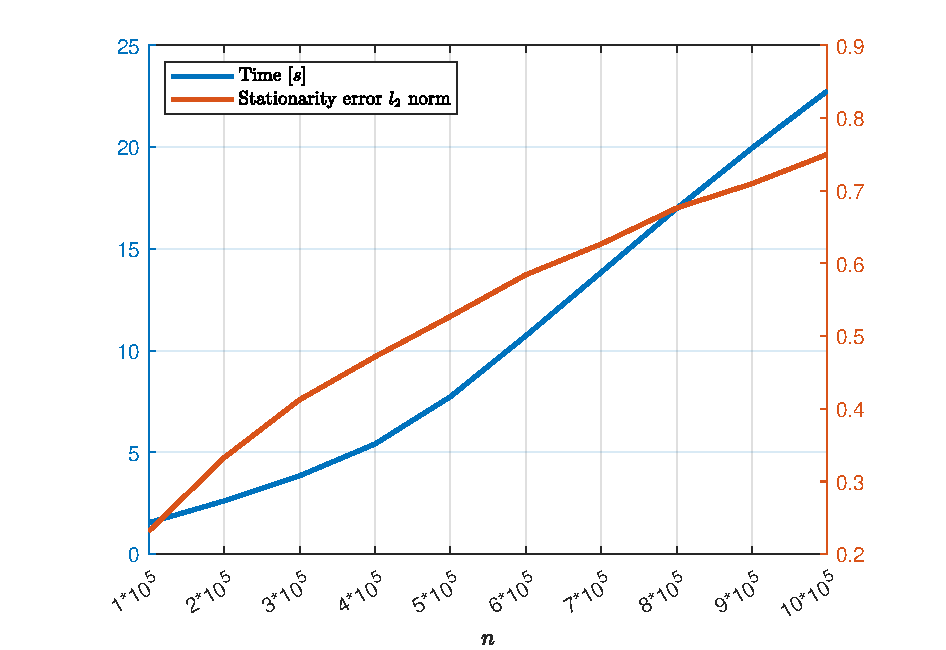
\includegraphics[scale = 0.45]{pictures/augmented_native.pdf}}
    \subfloat[2][Our GMRES implementation]{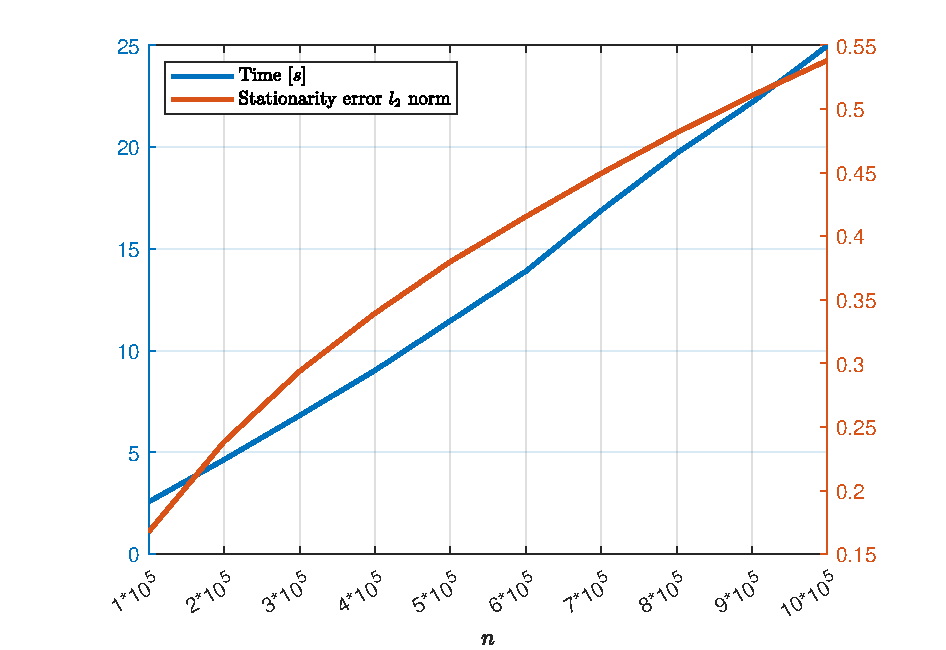
\includegraphics[scale = 0.45]{pictures/augmented_v1.pdf}}
    \caption{Time and stationarity error of the IPM algorithm using the native GMRES function implemented in MATLAB and our implementation shown for different values of \(n\).}
    \label{time_accuracy}
  \end{figure}

\noindent In \ref{time_accuracy} we can see that both computational time and accuracy of the method scale roughly linearly with the dimension of the problem. As a measure of accuracy we used the error on the stationarity condition as defined in \ref{Sec1_Eq_kkt_after}, in particular:
\[ \| Qx + c - \hat{A}^T \hat{\lambda} \| _ 2\]

\noindent A very important note is the fact that using an iterative linear system solver is \textbf{the only way to perform IPM at large scale}. We tried to solve the linear systems involved in the IPM iterations using the \textit{Backslash operator} in MATLAB (which is the standard operator to solve linear systems) but this resulted in \textbf{failing the test} when the dimension of the problem approaches \(n \sim 10^5\). Not only computational times are much higher (\(\sim 1\)min for the backslash versus \(\sim 1\)sec for the GMRES when \(n \sim 10^5\) ) but the backslash operator cannot handle the dimension of the linear system returning \texttt{NaN} as results. This could be due to the conditioning of the matrices and the lack of enough RAM memory in the system.
\\
\\
\noindent The fact that we can solve such algorithm with enough accuracy only by using an iterative linear system solver is made possible because the solution of the linear systems at each iteration does not need to be much accurate itself. The GMRES algorithm in fact stops without reaching the desired tolerance most of the time, but this is not a problem for the accuracy of the final solution. Moreover, since the maximum iterations of the GMRES algorithm are fixed, bad conditioning of the matrix does not affect computational times unlike  with the backslash operator.

\begin{figure}[H]
	\centering
	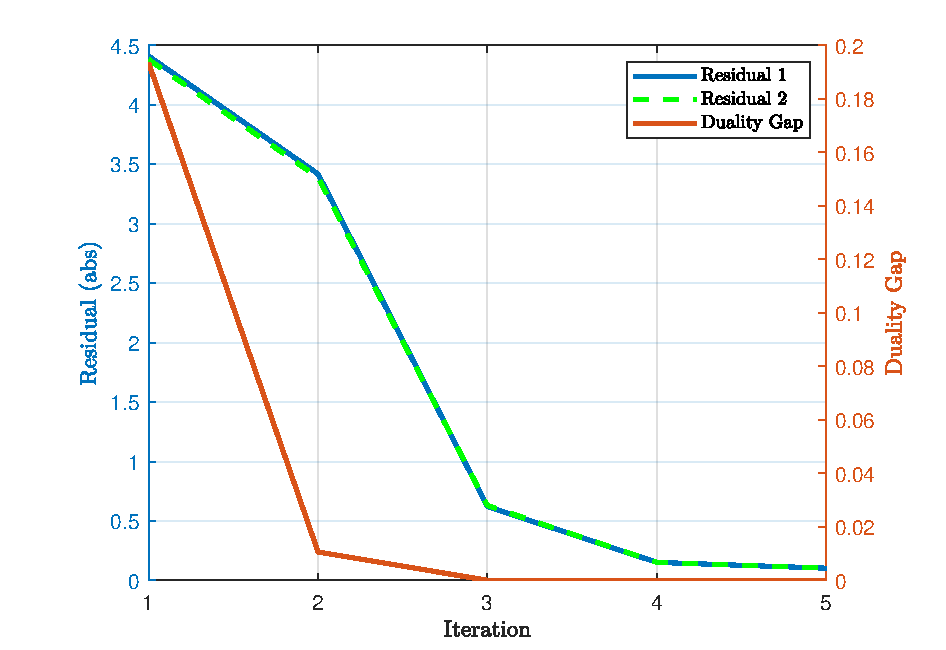
\includegraphics[scale = 0.8]{pictures/res_vs_duality.pdf}
	\caption{Residuals relative to the computation of both linear systems in each step of the IPM algorithm compared to the duality gap evolution. \(n = 10^6\), \(K = 100\)}
	\label{res_vs_duality}
\end{figure}

\noindent Since we can compute the duality gap at each step \(k\) of the IPM algorithm as:
\[
	\text{Duality Gap} = (2K + n)\mu_k
\]
We can compare it to the residuals of the solutions of both linear systems in each iteration that can be easily retrieved from the GMRES algorithm as in INSERISCI REFERENCE A RESIDUO GMRES. As we can se in Figure \ref{res_vs_duality} the the magnitude of the absolute residual of both linear systems is small enough to  guarantee the convergence of the IPM algorithm in 5 iterations and the duality gap to be basically zero. 



\end{document}